\section{TIẾP TUYẾN CỦA ĐƯỜNG TRÒN} % Tên bài
\subsection{Tiếp tuyến của đường tròn}
\subsubsection{Kiến thức trọng tâm}
\begin{tomtat}
	\begin{itemize}
		\item Dấu hiệu nhận biết tiếp tuyến của đường tròn \\
		Một đường thẳng là tiếp tuyến của đường tròn khi nó đi qua một điểm của đường tròn và vuông góc với bán kính đi qua điểm đó.
		\item Tính chất của hai tiếp tuyến cắt nhau\\
		Nếu hai tiếp tuyến của một đường tròn cắt nhau tại một điểm thì:
		\begin{itemize}
			\item Điểm đó cách đều hai tiếp điểm.
			\item Tia kẻ từ điểm đó đi qua tâm là tia phân giác của góc tạo bởi hai tiếp tuyến.
			\item Tia kẻ từ tâm đi qua điểm đó là tia phân giác của góc tạo bởi hai bán kính đi qua các tiếp điểm.
		\end{itemize}
	\begin{center}
	    \begin{tikzpicture}[line join = round, line cap=round,>=stealth,font=\footnotesize,scale=1]
	        \def \r{2.5} 
	        \path 
	        (0,0) coordinate (I)
	        (120:\r) coordinate (E)
	        (-120:\r) coordinate (F)
	        (-4.6,0) coordinate (M)
	        ; 
	        \foreach \diem in {I,E,F,M}
	        \draw[fill=black] (\diem);
	        \draw (I) circle(\r cm);
	        
	        % --- PHẦN SỬA ĐỔI ---
	        % Thay vì vẽ tất cả các đường bằng một lệnh, ta vẽ ME và MF riêng
	        % để thêm ký hiệu bằng nhau.
	        \draw (M) -- (E) node[midway, sloped] {$|$};
	        \draw (M) -- (F) node[midway, sloped] {$|$};
	        % Vẽ các đường còn lại
	        \draw (E)--(I)--(F)--(M)--(I);
	        % --- KẾT THÚC SỬA ĐỔI ---
	        
	        \pic [draw, line cap=round, angle eccentricity=0.6, angle radius=2mm] {right angle = M--E--I};
	        \pic [draw, line cap=round, angle eccentricity=0.6, angle radius=2mm] {right angle = M--F--I};
	        
	        \begin{scope}
	        \clip (E)--(I)--(M);
	        \draw (I) circle(10pt);
	        \end{scope}
	        
	        \begin{scope}
	        \clip (F)--(I)--(M);
	        \draw (I) circle(10pt);
	        \end{scope}
	        
	        \begin{scope}
	        \clip (E)--(M)--(I);
	        \draw (M) circle(10pt);
	        \draw (M) circle(7pt);
	        \end{scope}
	        
	        \begin{scope}
	        \clip (F)--(M)--(I);
	        \draw (M) circle(10pt);
	        \draw (M) circle(7pt);
	        \end{scope}
	    \end{tikzpicture}
	\end{center}
	\end{itemize}
\end{tomtat}

\begin{vd}%[Dự án Tài liệu Toán 9]%[Trần Tiến Đức]%[9H2N2-2]
	Cho $\triangle ABC$ có ba góc nhọn, kẻ đường cao $AH$, vẽ đường tròn $(A;AH)$. Chứng minh $BC$ là tiếp tuyến của đường tròn $(A;AH)$.
	\loigiai{
		\begin{center}
			\begin{tikzpicture}[line join = round, line cap=round,>=stealth,font=\footnotesize,scale=1]
				\def \r{2.5} 
				\path 
				(0,0) coordinate (A)
				(2,-\r) coordinate (C)
				(-1,-\r) coordinate (B)
				($(B)!(A)!(C)$)coordinate (H)
				; 
				\foreach \diem/\vitri in {A/90,C/-90,B/-90,H/-90}
				\draw[fill=black] (\diem) circle(1pt) node[shift={
					(\vitri:3mm)
				}]{$\diem$};
				\draw (A) circle(\r cm);
				\draw (A)--(B)--(C)--cycle;
				\draw (A)--(H);
				
				\pic [draw, line cap=round, angle eccentricity=0.6, angle radius=2mm] {right angle = A--H--C};
			\end{tikzpicture}
		\end{center}
		Xét đường tròn $(A;AH)$ có $AH \perp BC$ tại $H$ nên $BC$ là tiếp tuyến của $(A;AH)$. 
		}
\end{vd}

\begin{vd}%[Dự án Tài liệu Toán 9]%[Trần Tiến Đức]%[9H2N2-2]
	Cho đường tròn $(O;R)$ đường kính $AB$. Vẽ dây $BC$ sao cho $BC=R$. Trên tia đối của tia $BA$ lấy điểm $M$	sao cho $BM=R$. Chứng minh $MC$ là tiếp tuyến của đường tròn $(O;R)$.
	\loigiai{
		\begin{center}
			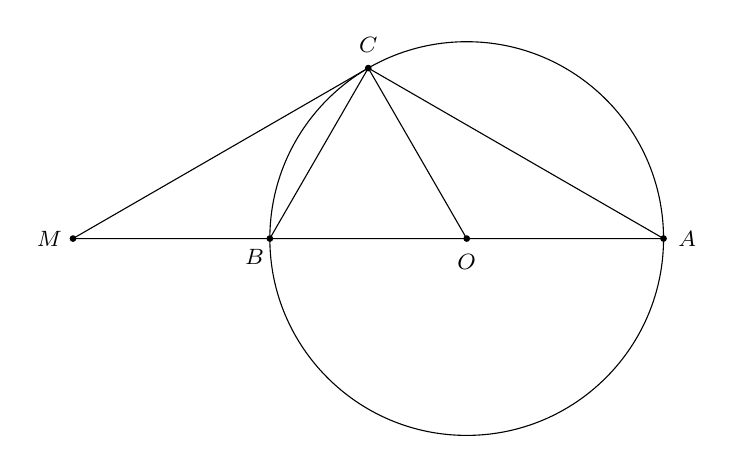
\begin{tikzpicture}[line join = round, line cap=round,>=stealth,font=\footnotesize,scale=1]
				\def \r{2.5} 
				\path 
				(0,0) coordinate (O)
				(0:\r) coordinate (A)
				(180:\r) coordinate (B)
				(-1.25,2.165) coordinate (C)
				(-5,0) coordinate (M)
				; 
				\foreach \diem/\vitri in {O/-90,M/180,C/90,B/-130,A/0}
				\draw[fill=black] (\diem) circle(1pt) node[shift={
					(\vitri:3mm)
				}]{$\diem$};
				\draw (O) circle(\r cm);
				\draw (A)--(B)--(C)--cycle;
				\draw (B)--(M)--(C)--(O);
			\end{tikzpicture}
		\end{center}
		Xét $\triangle MCO$ có \\
		$CB$ là trung tuyến ($MB=BO$)\\
		$CB=MB=BO=\dfrac{MO}{2}$\\
		Nên $\triangle MCO$ vuông tại $C$ hay $MC \perp CO$.\\
		Xét đường tròn $(O;R)$ có  $MC \perp CO$ tại $C$ nên $MC$ là tiếp tuyến của $(O;R)$. 
			}
\end{vd}

\begin{vd}%[Dự án Tài liệu Toán 9]%[Trần Tiến Đức]%[9H2H2-2]
	Cho điểm $E$ thuộc nửa đường tròn tâm $O$, đường kính $MN$. Kẻ tiếp tuyến tại $N$ của đường tròn tâm $O$, tiếp tuyến này cắt đường thẳng $ME$ tại $D$. Chứng minh $\triangle MEN$ vuông tại $E$. Từ đó chứng minh $DE \cdot DM = DN^2$.
	\loigiai{
		\begin{center}
			\begin{tikzpicture}[line join = round, line cap=round,>=stealth,font=\footnotesize,scale=1]
				\def \r{2.5} 
				\path 
				(0,0) coordinate (O)
				(0:\r) coordinate (N)
				(2.5,5) coordinate (N1)
				(180:\r) coordinate (M)
				(70:\r) coordinate (E)
				(intersection of M--E and N--N1) coordinate (D) 
				; 
				\foreach \diem/\vitri in {O/-90,M/180,N/0,E/90,D/0}
				\draw[fill=black] (\diem) circle(1pt) node[shift={
					(\vitri:3mm)
				}]{$\diem$};
				\draw (O) circle(\r cm);
				\draw (M)--(N)--(D)--cycle;
				\draw (O)--(E)--(N);
				
				\pic [draw, line cap=round, angle eccentricity=0.6, angle radius=2mm] {right angle = M--N--D};
			\end{tikzpicture}
		\end{center}
		$\triangle MEN$ có $OM = ON = OE = \dfrac{MN}{2}$ nên $\triangle MEN$ vuông tại $E$.\\
		Xét đường tròn $(O)$ có $DN$ là tiếp tuyến tại $N$ nên $DN \perp MN$ hay $\widehat{DNM}= 90^\circ$.\\
		Xét hai tam giác $\triangle DEN$ và $\triangle DNM$ có\\
		$\widehat{DEN} = \widehat{DNM }= 90^\circ$\\
		$\widehat{MDN}$ là góc chung\\
		Nên $\triangle DEN \sim \triangle DNM$ (g.g)\\
		Suy ra $\dfrac{DE}{DN} = \dfrac{DN}{DM}$ hay $DE \cdot DM = DN^2$.
	}
\end{vd}

\begin{vd}%[Dự án Tài liệu Toán 9]%[Trần Tiến Đức]%[9H2H2-3]
	Cho điểm $M$ nằm ngoài đường tròn $I$ và $ME$, $MF$ là hai tiếp tuyến của đường tròn tại $E$ và $F$. Biết $\widehat{EMF}=60^\circ$. Tính $\widehat{EMI}$ và $\widehat{EIF}$.
	\loigiai{
	\begin{center}
		\begin{tikzpicture}[line join = round, line cap=round,>=stealth,font=\footnotesize,scale=1]
			\def \r{2.5} 
			\path 
			(0,0) coordinate (I)
			(120:\r) coordinate (E)
			(-120:\r) coordinate (F)
			(-4.6,0) coordinate (M)
			; 
			\foreach \diem/\vitri in {I/0,E/90,F/-90,M/180}
			\draw[fill=black] (\diem) circle(1pt) node[shift={
				(\vitri:3mm)
			}]{$\diem$};
			\draw (I) circle(\r cm);
			\draw (M)--(E)--(I)--(F)--(M)--(I);
			\draw ;
			
			\pic [draw, line cap=round, angle eccentricity=0.6, angle radius=2mm] {right angle = M--E--I};
			\pic [draw, line cap=round, angle eccentricity=0.6, angle radius=2mm] {right angle = M--F--I};
		\end{tikzpicture}
	\end{center}
		Vì $ME$, $MF$ là hai tiếp tuyến của đường tròn $(I)$ tại $E$ và $F$ nên $MI$ là phân giác của $\widehat{EMF}$ và $\widehat{EIF}$.\\
		Suy ra $\widehat {EMI} = \widehat {FMI} = \dfrac{1}{2}\widehat{EMF} = 30^\circ$ và $\widehat {EIM} = \widehat {FIM} = \dfrac{1}{2}\widehat {FIE}$.\\
		Xét $\triangle EIM$ vuông tại $E$ (vì $ME$ là tiếp tuyến của đường tròn tại $E$) có $\widehat {EIM} = 90^\circ - \widehat{EMI} = 60^\circ$.\\
		Suy ra $\widehat {EIF} = 2\widehat {EIM} = 120^\circ$.
	}
\end{vd}

\begin{vd}%[Dự án Tài liệu Toán 9]%[Trần Tiến Đức]%[9H2N2-3]
	Cho đường tròn $(O;R)$. Từ điểm $M$ nằm ngoài đường tròn kẻ hai tiếp tuyến $MA$, $MB$ tới đường tròn ($A$, $B$ là các tiếp điểm). Chứng minh $OM \perp AB$.
	\loigiai{
		\begin{center}
			\begin{tikzpicture}[line join = round, line cap=round,>=stealth,font=\footnotesize,scale=1]
				\def \r{2.5} 
				\path 
				(0,0) coordinate (O)
				(120:\r) coordinate (A)
				(-120:\r) coordinate (B)
				(-4.6,0) coordinate (M)
				($(M)!1/2!(O)$)coordinate (I)
				; 
				\foreach \diem/\vitri in {O/0,A/90,B/-90,M/180,I/-110}
				\fill (\diem) circle(1.5pt) node[shift={
					(\vitri:3mm)
				}]{$\diem$};
				\draw (O) circle(\r cm);
				\draw (M)--(A)--(O)--(B)--(M)--(O);
				\draw (A)--(I)--(B)--cycle;
				
				\pic [draw, line cap=round, angle eccentricity=0.6, angle radius=2mm] {right angle = M--A--O};
				\pic [draw, line cap=round, angle eccentricity=0.6, angle radius=2mm] {right angle = M--B--O};
			\end{tikzpicture}
		\end{center}
		Xét $(O)$ có $MA$, $MB$ là hai tiếp tuyến cắt nhau tại $M$.\\
					Suy ra $MA = MB$ nên $M$ thuộc trung trực của $AB$.\\
					Có $OA = OB$ nên $O$ thuộc trung trực của $AB$.\\ 
					Suy ra $MO$ là trung trực của $AB$.\\
					Suy ra $MO \perp AB$.
	}
\end{vd}

\begin{vd}%[Dự án Tài liệu Toán 9]%[Trần Tiến Đức]%[9H2H2-3]
	Cho nửa đường tròn $(O)$ đường kính $AB$. Trên nửa mặt phẳng bờ $AB$ chứa nửa đường tròn vẽ các tiếp tuyến $Ax$ và $By$. Điểm $M$ thuộc $(O)$ sao cho tiếp tuyến tại $M$ cắt $Ax$, $By$ lần lượt tại $C$, $D$. Chứng minh $\triangle COD$ vuông tại $O$.
	\loigiai{
		\begin{center}
			\begin{tikzpicture}[line join = round, line cap=round,>=stealth,font=\footnotesize,scale=1]
				\def \r{2.5} 
				\path 
				(0,0) coordinate (O)
				(180:\r) coordinate (A)
				(0:\r) coordinate (B)
				(-2.5,5) coordinate (A1)
				(2.5,5) coordinate (B1)
				(110:\r) coordinate (M)
				(-2.5,1.65) coordinate (C)
				(2.5,3.8) coordinate (D)
%				($(M)!1/2!(O)$)coordinate (I)
				; 
				\foreach \diem/\vitri in {O/-90,A/180,B/0,M/90,C/180,D/0}
				\draw[fill=black] (\diem) circle(1pt) node[shift={
					(\vitri:3mm)
				}]{$\diem$};
				\draw (O) -- (A) arc (180:0:\r) -- cycle;
				\draw (A)--(A1) (B)--(B1);
				\draw (O)--(M) (O)--(C) (O)--(D);
				\draw (C)--(D);
				
				\pic [draw, line cap=round, angle eccentricity=0.6, angle radius=2mm] {right angle = C--A--O};
				\pic [draw, line cap=round, angle eccentricity=0.6, angle radius=2mm] {right angle = O--B--D};
				\pic [draw, line cap=round, angle eccentricity=0.6, angle radius=2mm] {right angle = O--M--D};
			\end{tikzpicture}
		\end{center}
		Xét đường tròn $(O)$ có $CA$, $CM$ là hai tiếp tuyến tại $A$ và $M$ nên $OC$ là tia phân giác của $\widehat{AOM}$.\\
		Hay $\widehat{COM}=\dfrac{1}{2}\widehat{AOM}$.\\
		Xét đường tròn $(O)$ có $DB$, $DM$ là hai tiếp tuyến tại $B$ và $M$ nên $OD$ là tia phân giác của $\widehat{MOB}$.\\
		Hay $\widehat{MOD}=\dfrac{1}{2}\widehat{MOB}$.\\
		Có $\widehat{COD}=\widehat{COM}+\widehat{MOD}=\dfrac{1}{2}\widehat{AOM}+\dfrac{1}{2}\widehat{MOB}=\dfrac{1}{2} \cdot 180^\circ=90^\circ$.\\
		Xét $\triangle COD$ có $\widehat{COD}=90^\circ$ nên $\triangle COD$ vuông tại $C$.
		}
\end{vd}

\subsubsection{Bài tập}
\begin{bt}%[Dự án Tài liệu Toán 9]%[Trần Tiến Đức]%[9H2H2-2]
	Cho $\triangle ABC$ vuông tại $A$, kẻ đường cao $AH$. Gọi $M$ là trung điểm của $AB$. Chứng minh $MH$ là tiếp tuyến của đường tròn $\left(O; \dfrac{AC}{2}\right)$.
	\loigiai{
		\begin{center}
			\begin{tikzpicture}[line join = round, line cap=round,>=stealth,font=\footnotesize,scale=0.8]
				\def \r{2.5} 
				\path 
				(0,0) coordinate (O)
				(-4,0) coordinate (A)
				(-4,6) coordinate (B)
				(4,0) coordinate (C)
				($(B)!(A)!(C)$)coordinate (H)
				($(A)!1/2!(B)$)coordinate (M)
				; 
				\foreach \diem/\vitri in {O/-90,A/-135,M/180,B/-135,H/90,C/-45}
				\draw[fill=black] (\diem) circle(1pt) node[shift={
					(\vitri:3mm)
				}]{$\diem$};
				\draw (A)--(B)--(C)--cycle;
				\draw (H)--(A) (H)--(M) (H)--(O);
				
				\pic [draw, line cap=round, angle eccentricity=0.6, angle radius=2mm] {right angle = A--H--C};
			\end{tikzpicture}
		\end{center}
		Xét $\triangle AHC$ vuông tại $H$ ($AH \perp BC$) có $O$ là trung điểm của $AC$ (gt).\\
		Suy ra $HO$ là đường trung tuyến ứng với $AC$.\\
		Suy ra $HO = AO = OC = \frac{1}{2} AC$.\\
		Xét $\triangle AOH$ có $HO=AO$ nên $\triangle AOH$ cân tại $O$.
		Suy ra  $\widehat{OAH} =\widehat{OHA}$.\\
		Xét tam giác $\triangle AHB$ vuông tại $H$ ($AH \perp BC$) có $M$ là trung điểm của $AB$ (gt).\\
		Suy ra $HM$ là đường trung tuyến ứng với $AB$.\\
		Suy ra $HM = MB = MA = \frac{1}{2} AB$.\\
		Xét $\triangle MHA$ có $HM=MA$ nên $\triangle MHA$ cân tại $M$.
		Suy ra $\widehat{MHA} = \widehat{MAH}$.\\
		Ta có $\widehat{MHO} = \widehat{MHA} +\widehat{AHO} = \widehat{MAH} + \widehat{OAH} = \widehat{MAO} = \widehat{BAC} = 90^\circ$\\
		Suy ra $MH \perp HO$.\\
		Suy ra $MH$ là tiếp tuyến của đường tròn $\left(O; \frac{AC}{2}\right)$.
	}
\end{bt}

\begin{bt}%[Dự án Tài liệu Toán 9]%[Trần Tiến Đức]%[9H2N2-2]
	Cho đường tròn $(O; R)$ có đường kính $AB$. Vẽ dây $AC$ sao cho $\widehat{CAB} = 30^\circ$ và $\widehat{ACB} = 90^\circ$. Lấy điểm $M$ sao cho $B$ là trung điểm của đoạn thẳng $OM$. Chứng minh $MC$ là tiếp tuyến của đường tròn $(O)$.
	\loigiai{
		\begin{center}
			\begin{tikzpicture}[line join = round, line cap=round,>=stealth,font=\footnotesize,scale=0.8]
				\def \r{2.5} 
				\path 
				(0,0) coordinate (O)
				(180:\r) coordinate (A)
				(0:\r) coordinate (B)
				(60:\r) coordinate (C)
				(5,0) coordinate (M)
				; 
				\foreach \diem/\vitri in {O/-90,A/180,M/-90,B/-35,C/90}
				\draw[fill=black] (\diem) circle(1pt) node[shift={
					(\vitri:3mm)
				}]{$\diem$};
				\draw (O) circle(\r cm);
				\draw (A)--(C)--(M)--cycle;
				\draw (O)--(C)--(B);
				
				\pic [draw, line cap=round, angle eccentricity=0.6, angle radius=2mm] {right angle = A--C--B};
			\end{tikzpicture}
		\end{center}
		Xét $\triangle ABC$ có $\widehat{ACB} = 90^\circ$ nên $\triangle ABC$ vuông tại $C$.
		Mà $\widehat{ACO} = 30^\circ$.\\
		Suy ra $\widehat{OCB} = 60^\circ$.\\
		Xét $\triangle OBC$ cân tại $O$ suy ra $\triangle OBC$ đều hay $BC = OB = \dfrac{OM}{2}$.\\
		Do đó $\triangle OCM$ vuông tại $C$ hay $MC \perp OC$ tại $C$.\\
		Vậy $MC$ là tiếp tuyến của đường tròn $(O)$.
	}
\end{bt}

\begin{bt}%[Dự án Tài liệu Toán 9]%[Trần Tiến Đức]%[9H2H2-3]
	Cho đường tròn tâm $O$ có bán kính $OA = R$, dây $BC \perp OA$ tại trung điểm $M$ của $OA$. Kẻ tiếp tuyến của đường tròn tại $B$, cắt đường thẳng $OA$ tại $E$. Tính độ dài $BE$ theo $R$.
	\loigiai{
		\begin{center}
			\begin{tikzpicture}[line join = round, line cap=round,>=stealth,font=\footnotesize,scale=1]
				\def \r{2.5} 
				\path 
				(0,0) coordinate (O)
				(180:\r) coordinate (A)
				(120:\r) coordinate (B)
				(-120:\r) coordinate (C)
				(intersection of B--C and A--O) coordinate (M) 
				(-4.6,0) coordinate (E)
				; 
				\foreach \diem/\vitri in {O/0,M/-135,C/-90,B/90,A/-135,E/180}
				\draw[fill=black] (\diem) circle(1pt) node[shift={
					(\vitri:3mm)
				}]{$\diem$};
				\draw (O) circle(\r cm);
				\draw (O)--(B)--(A)--(C)--(O);
				\draw (O)--(E)--(B) (B)--(C);
				
				\pic [draw, line cap=round, angle eccentricity=0.6, angle radius=2mm] {right angle = E--B--O};
				\pic [draw, line cap=round, angle eccentricity=0.6, angle radius=2mm] {right angle = B--M--O};
			\end{tikzpicture}
		\end{center}
		Vì $OA = R$ nên $OM = \dfrac{R}{2}$.\\
		
		Xét $\triangle OBE$ và $\triangle OMB$ có\\
		$\widehat{EBO}= \widehat{BMO}$\\
		$\widehat{BOE}$ là góc chung\\
		Nên $\triangle OBE \sim \triangle OMB$ (g.g)\\ 
		Suy ra $\dfrac{OB}{OM} = \dfrac{OE}{OB}$ \\
		Hay $OE = \dfrac{OB^2}{OM} = \dfrac{R^2}{\dfrac{R}{2}} = 2R$.\\
		
		Xét $\triangle AOB$ có $MB$ là đường cao, đường trung tuyến nên $\triangle AOB$ cân tại $B$.\\
		Xét $\triangle AOB$ cân tại $B$ có $OA=OB(=R)$ nên $\triangle AOB$ là tam giác đều.\\
		Suy ra $\widehat{BOA}=60^\circ$ hay $\widehat{BOE}=60^\circ$.\\
		Xét đường tròn $(O)$ có $EB$ là tiếp tuyến tại $B$ nên $EB \perp OB$ hay $\widehat{EBO}= 90^\circ$.\\
		Xét $\triangle OBE$ vuông tại $B$  ta có
		\begin{eqnarray*}
		\tan\widehat{BOE}&=& \dfrac{BE}{OB}\\
		\tan60^\circ&=& \dfrac{BE}{R}\\
		\sqrt{3}&=&\dfrac{BE}{R}\\
		BE&=&R\sqrt{3}.
		\end{eqnarray*}
	}
\end{bt}

\begin{bt}%[Dự án Tài liệu Toán 9]%[Trần Tiến Đức]%[9H2V2-3]
	Cho đường tròn $(O,R)$ có dây $AB$ không là đường kính. Qua $O$ kẻ đường thẳng vuông góc với $AB$, cắt tiếp tuyến tại $A$ của $(O)$ ở điểm $C$.
	\begin{itemize}
		\item[a)] Chứng minh $CB$ là tiếp tuyến của $(O)$.
		\item[b)] Tính độ dài đoạn thẳng $OC$, biết $R=15 \text{ cm}$ và $AB=24 \text{ cm}$.
	\end{itemize}
	\loigiai{
		\begin{center}
			\begin{tikzpicture}[line join = round, line cap=round,>=stealth,font=\footnotesize,scale=1]
				\def \r{2.5} 
				\path 
				(0,0) coordinate (O)
				(60:\r) coordinate (A)
				(-60:\r) coordinate (B)
				(5,0) coordinate (C)
				(intersection of A--B and C--O) coordinate (H) 
				; 
				\foreach \diem/\vitri in {O/180,H/45,C/0,B/-90,A/90}
				\draw[fill=black] (\diem) circle(1pt) node[shift={
					(\vitri:3mm)
				}]{$\diem$};
				\draw (O) circle(\r cm);
				\draw (A)--(B)--(C)--cycle;
				\draw (C)--(O) (B)--(O) (A)--(O);
				
				\pic [draw, line cap=round, angle eccentricity=0.6, angle radius=2mm] {right angle = O--A--C};
				\pic [draw, line cap=round, angle eccentricity=0.6, angle radius=2mm] {right angle = O--H--A};
				\path (0,0) node{\hypersetup{hidelinks}\href{RAJSO3u}{ }};
			\end{tikzpicture}
		\end{center}
		\begin{itemize}
			\item[a)] Gọi $H$ là giao điểm của $AB$ và $OC$.\\
			Vì $A, B \in (O;R)$ suy ra $OA=OB$.\\
			Xét $\triangle OAB$ có $OA=OB$ nên $\triangle OAB$ cân tại $O$.\\
			Mà $OH \perp AB$ tại $H$.\\
			Nên $OH$ là đường cao, trung trực, phân giác của $\triangle OAB$.\\
			Suy ra $\widehat{AOH} = \widehat{BOH}$ hay $\widehat{AOC} = \widehat{BOC}$.\\
			Xét $\triangle OAC$ và $\triangle OBC$ có\\
			$OA=OB (=R)$;\\
			$\widehat{AOC} = \widehat{BOC}$ (cmt);\\
			$OC$ chung.\\
			Nên $\triangle OAC = \triangle OBC$ (c.g.c).\\
			Suy ra $\widehat{OAC} = \widehat{OBC}=90^\circ$ (2 góc tương ứng) hay $OB \perp BC$.\\
			Xét đường tròn $(O;R)$ có $B \in (O;R)$ và $OB \perp BC$ tại $B$.\\
			Suy ra $CB$ là tiếp tuyến của đường tròn $(O;R)$.
			\item[b)] Xét $\triangle OAB$ cân tại $O$ có $OH$ là đường trung tuyến ứng với cạnh $AB$\\
			Suy ra $HA = HB = \frac{AB}{2} = \frac{24}{2} = 12$ (cm).\\
			Xét $\triangle OAH$ vuông tại $H$  ($OH \perp AB$) theo Pythagore, ta có
			\begin{eqnarray*}
				OA^2 &=& AH^2 + OH^2\\
				15^2 &=& 12^2 + OH^2\\
				OH^2 &=& 15^2 - 12^2\\
				OH &=& 9 \text{ (cm)}.
			\end{eqnarray*}
			Xét $\triangle OAH$ vuông tại $H$ có $\widehat{HOA}+\widehat{OAH}=90^\circ$.\\
			Mà $\widehat{OAH}+\widehat{HAC}=90^\circ$.\\
			Suy ra $\widehat{HOA}=\widehat{HAC}$.\\
			Xét $\triangle HOA$ vuông tại $H$ và $\triangle HAC$ vuông tại $H$ có\\
			 $\widehat{HOA}=\widehat{HAC}$.\\
			Nên  $\triangle HOA \sim \triangle HAC$ (g.g)\\
			Suy ra \\
			\begin{eqnarray*}
				\dfrac{AH}{OH} &=& \dfrac{CH}{AH} \text{ (2 cặp cạnh tương ứng tỉ lệ)}\\
				AH^2 &=& OH \cdot CH\\
				12^2 &=& 9 \cdot CH\\
				CH &=& 16 \text{ (cm)}.
			\end{eqnarray*}
			Ta có $OC = OH + HC = 9 + 16 = 25$(cm).
		\end{itemize}
	}
\end{bt}

\begin{bt}%[Dự án Tài liệu Toán 9]%[Trần Tiến Đức]%[9H2H2-3]
	Cho $\triangle ABC$ có đường tròn $(O)$ nằm trong và tiếp xúc với $AB$ tại $M$, $BC$ tại $P$, $AC$ tại $E$. Biết $AM=6$ cm, $BP=3$ cm, $CE=8$ cm. Tính chu vi tam giác $ABC$.
	\loigiai{
		\begin{center}
			\begin{tikzpicture}[line join = round, line cap=round,>=stealth,font=\footnotesize,scale=0.5]
				\def \r{3} 
				\path 
				(0,0) coordinate (O)
				(180:\r) coordinate (M)
				(-90:\r) coordinate (P)
				(45:\r) coordinate (E)
				(-3,-3) coordinate (B)
				(-3,6.6) coordinate (A)
				(8,-3) coordinate (C)
				; 
				\foreach \diem/\vitri in {O/0,A/90,M/180,B/-135,P/-90,C/-45,E/45}
				\draw[fill=black] (\diem) circle(2.5pt) node[shift={
					(\vitri:3mm)
				}]{$\diem$};
				\draw (O) circle(\r cm);
				\draw (A)--(B)--(C)--cycle;
				\draw (M)--(O) (P)--(O) (E)--(O);
				
				\pic [draw, line cap=round, angle eccentricity=0.6, angle radius=2mm] {right angle = A--M--O};
				\pic [draw, line cap=round, angle eccentricity=0.6, angle radius=2mm] {right angle = O--P--C};
				\pic [draw, line cap=round, angle eccentricity=0.6, angle radius=2mm] {right angle = O--E--C};
			\end{tikzpicture}
		\end{center}
		$AE, AM$ là hai tiếp tuyến của $(O)$ cắt nhau tại $A$ nên $AE = AM = 6$ (cm) (tính chất hai tiếp tuyến cắt nhau).\\
		$BM, BP$ là hai tiếp tuyến của $(O)$ cắt nhau tại $B$ nên $BM = BP = 3 $ (cm) (tính chất hai tiếp tuyến cắt nhau).\\
		$CP, CE$ là hai tiếp tuyến của $(O)$ cắt nhau tại $C$ nên $CP = CE = 8$ (cm) (tính chất hai tiếp tuyến cắt nhau).\\
		Chu vi tam giác ABC là
		$AB + BC + CA = AM + BM + BP + CP + CE + AE = 6+3+3+8+8+6 = 34 $ (cm).
	}
\end{bt}

